\documentclass{article}
\usepackage{geometry}
\geometry{a4paper, top=3cm, bottom=3cm, left=3.5cm, right=3.5cm, heightrounded, bindingoffset=5mm}

%\documentclass[12pt, letterpaper, twoside]{article}
\usepackage[utf8]{inputenc}




\renewcommand{\contentsname}{Indice}

\usepackage{algpseudocode}
\usepackage{hyperref}
\usepackage{amsmath}
\usepackage{caption}
\usepackage{float}
\usepackage{enumitem}
\hypersetup{hidelinks}
% Sillabazione italiana
\usepackage[italian]{babel}
%\usepackage{authblk}
% Json format
%\usepackage{bera}% optional: just to have a nice mono-spaced font
\usepackage{listings}
\usepackage{xcolor}

\colorlet{punct}{red!60!black}
\definecolor{background}{HTML}{EEEEEE}
\definecolor{delim}{RGB}{20,105,176}
\colorlet{numb}{magenta!60!black}

\lstdefinelanguage{json}{
    basicstyle=\normalfont\ttfamily,
    numbers=left,
    numberstyle=\scriptsize,
    stepnumber=1,
    numbersep=6pt,
    showstringspaces=false,
    breaklines=true,
    frame=lines,
    backgroundcolor=\color{background},
    literate=
     *{0}{{{\color{numb}0}}}{1}
      {1}{{{\color{numb}1}}}{1}
      {2}{{{\color{numb}2}}}{1}
      {3}{{{\color{numb}3}}}{1}
      {4}{{{\color{numb}4}}}{1}
      {5}{{{\color{numb}5}}}{1}
      {6}{{{\color{numb}6}}}{1}
      {7}{{{\color{numb}7}}}{1}
      {8}{{{\color{numb}8}}}{1}
      {9}{{{\color{numb}9}}}{1}
      {:}{{{\color{punct}{:}}}}{1}
      {,}{{{\color{punct}{,}}}}{1}
      {\{}{{{\color{delim}{\{}}}}{1}
      {\}}{{{\color{delim}{\}}}}}{1}
      {[}{{{\color{delim}{[}}}}{1}
      {]}{{{\color{delim}{]}}}}{1},
}

\usepackage{graphicx}
\graphicspath{ {./images/} }

% Remove algorithm number

\usepackage[linesnumbered,ruled,vlined]{algorithm2e}
\DontPrintSemicolon

\renewcommand{\KwSty}[1]{\textnormal{\textcolor{blue!90!black}{\ttfamily\bfseries #1}}\unskip}
\renewcommand{\ArgSty}[1]{\textnormal{\ttfamily #1}\unskip}
\SetKwComment{Comment}{\color{green!50!black}// }{}
\renewcommand{\CommentSty}[1]{\textnormal{\ttfamily\color{green!50!black}#1}\unskip}
\newcommand{\assign}{\leftarrow}
\newcommand{\var}{\texttt}
\newcommand{\Class}[2]{\texttt{\bfseries #1(#2)}}
\SetKwProg{Class}{class}{}{}
\newcommand{\With}[2]{\texttt{\bfseries #1(#2)}}
\SetKwProg{With}{with}{}{}
\newcommand{\FuncCall}[2]{\texttt{\bfseries #1(#2)}}
\SetKwProg{Function}{function}{}{}
\renewcommand{\ProgSty}[1]{\texttt{\bfseries #1}}

\title{\textbf{Progetto Finale Big Data}}
%\author[1] {Manuel Granchelli}
%\affil[1]{Dipartimento di Ingegneria Informatica, Università degli Studi Roma Tre}
\date{}

\begin{document}
\maketitle

\begin{flushleft}
\textbf{Manuel Granchelli} 
\hfill {\href{mailto:man.granchelli@stud.uniroma3.it}{\textbf{man.granchelli@stud.uniroma3.it}}} \\
\textit{Matricola: 512406}\\
\textit{Dipartimento di Ingegneria Informatica}\\
\textit{Università degli Studi Roma Tre}\\
\par\bigskip
\textbf{Repo GitHub:} \href{https://github.com/mgranchelli/bigdata-finalproject}{https://github.com/mgranchelli/bigdata-finalproject}
\end{flushleft}

\section*{Introduzione}
In questo rapporto verranno illustrate le procedure di analisi, elaborazione, salvataggio e visualizzazione di dati catturati da sensori IoT installati in un campo di peschi. La strategia che usa le tecnologie dell'informazione per acquisire e monitorare i dati finalizzati alle decisioni per la produzione agricola è chiamata Agricoltura di Precisione. Lo scopo è quello di migliorare la produzione, minimizzare i danni ambientali ed elevare gli standard qualitativi dei prodotti agricoli.\\
Nel seguente caso, non avendo accesso diretto ai sensori sul campo, i dati sono stati raccolti per ogni sensore in un file diverso in formato JSON e tramite uno script Python è stato simulato il flusso streaming dei dati inviati dai sensori.
Lo script genera il flusso di dati e tramite Kafka invia messaggi a Spark Streaming che si occupa di processare i dati. Una volta processati i dati vengono salvati all'interno di un Time Series Database (TSDB). Questo perchè i dati prodotti dai sensori IoT sono tutti associati ad un timestamp e sono dati che devono essere monitorati nel tempo. I Time Series Database (TSDB) si prestano molto bene per essere utilizzati in queste situazioni e nel seguente progetto si è scelto di utilizzare InfluxDB. \\
I dati memorizzati vengono a loro volta letti da Grafana che è uno strumento di visualizzazione di serie temporali. Grafana è accessibile via browser dove è presente la dashboard contenente i grafici per monitorare i dati dei sensori memorizzati su InfluxDB. \\
L'architettura utilizzata in questo progetto è stata testata utilizzando docker compose che permette di realizzare applicazioni composte da più contenitori che comunicano tra di loro. Ogni contenitore è stato creato per svolgere una determinata attività con una determinata tecnologia. \\
Tutto il materiale utilizzato è disponibile nel repo GitHub:\\ \href{https://github.com/mgranchelli/bigdata-finalproject}{https://github.com/mgranchelli/bigdata-finalproject}.




\thispagestyle{empty}
\newpage

\tableofcontents
%\addcontentsline{toc}{section}{Unnumbered Section}

% Remove number page and start sections from this page
\thispagestyle{empty}

\clearpage
\pagenumbering{arabic}

\section{Dati Paradise}
I dati a disposizione sono stati catturati da 10 sensori installati in un campo di peschi. Questi dati sono stati raccolti in 10 file separati in formato JSON. I file utilizzati sono stati generati dai seguenti dispositivi:
\begin{itemize}[noitemsep]
  \item anemometer,
  \item anemometer2,
  \item humidity\_sensor,
  \item humidity\_sensor2,
  \item leaf\_wetness,
  \item leaf\_wetness2,
  \item rain\_sensor,
  \item solar\_radiation,
  \item thermometer,
  \item thermometer2.
\end{itemize}
Nel dettaglio:
\begin{itemize}[noitemsep]
  \item (\textbf{anemometer}, \textbf{anemometer2}): Anemometri, inviano dati relativi al vento. I dati raccolti sono: velocità minima (wind\_speed\_min), velocità massima (wind\_speed\_max) e direzione (wind\_dir) del vento,
  \item (\textbf{humidity\_sensor}, \textbf{humidity\_sensor2}): Sensori umidità, inviano dati relativi all'umidità dell'aria. I dati raccolti sono: umidità minima (humidity\_min) e umidità massima (humidity\_max).
  \item (\textbf{leaf\_wetness}, \textbf{leaf\_wetness2}): Bagnatura fogliare, inviano dati relativi alle condizioni di bagnatura delle superfici fogliari (rileva condensazione di particelle d'acqua sulla superficie delle foglie). I dati raccolti sono: bagnatura grezza superiore (top\_page\_raw) e inferiore delle foglie (bottom\_page\_raw) e bagnatura in percentuale superiore (top\_page\_perc) e inferiore delle foglie (bottom\_page\_perc).
  \item \textbf{rain\_sensor}: Pluviometro, invia dati relativi la pioggia (rain).
  \item \textbf{solar\_radiation}: Radiometro, invia dati relativi ai raggi solari (solar).
  \item (\textbf{thermometer}, \textbf{thermometer2}): Termo-igrometri, inviano dati relativi alla temperatura. I dati raccolti sono: temperatura minima (temperature\_min) e massima (temperature\_max).
\end{itemize}
\textbf{Esempio di file JSON (anemometer)}:
\begin{lstlisting}[language=json,firstnumber=1]
{
    "wind_speed_max": [
        {
            "ts": 1656369928000,
            "value": "14.39"
        }, ...
    ],
    "wind_speed_min": [
        {
            "ts": 1656369928000,
            "value": "1.93"
        }, ...
    ],
    "wind_dir": [
        {
            "ts": 1656369928000,
            "value": "79.0"
        }, ...
    ]
}
\end{lstlisting}

In ogni file JSON sono presenti i dati raccolti con le chiavi sopra citate. Per ogni chiave ci sono due valori: uno è il timestamp (ts) e l'altro è il valore catturato dal sensore (value). I dati a disposizioni sono stati raccolti nel periodo che va dal \date{01/04/2022}, al \date{27/06/2022}. 

I sensori inviano i dati ogni 15 minuti, quindi i dati presenti nei file JSON hanno intervalli di 15 minuti, tranne che per i sensori di bagnatura fogliare che inviano dati ogni minuto.

\newpage
\section{Architettura e tecnologie usate}
Lo scopo del seguente progetto è stato quello di analizzare i dati proventi da sensori IoT, processarli, salvarli all'interno di un database e visualizzarli su un browser in real time.
Per poter realizzare tutto il sistema è stato utilizzato docker compose che è uno strumento che consente di realizzare applicazioni composte da più contenitori che comunicano tra di loro. Sono stati creati vari contenitori, nei quali sono stati installati i servizi necessari per il funzionamento del sistema e collegati tra di loro tramite una rete virtuale che permette loro di interagire.
Nella seguente figura è possibile osservare schematicamente l'architettura del sistema realizzato con i relativi servizi.

\begin{figure}[H]
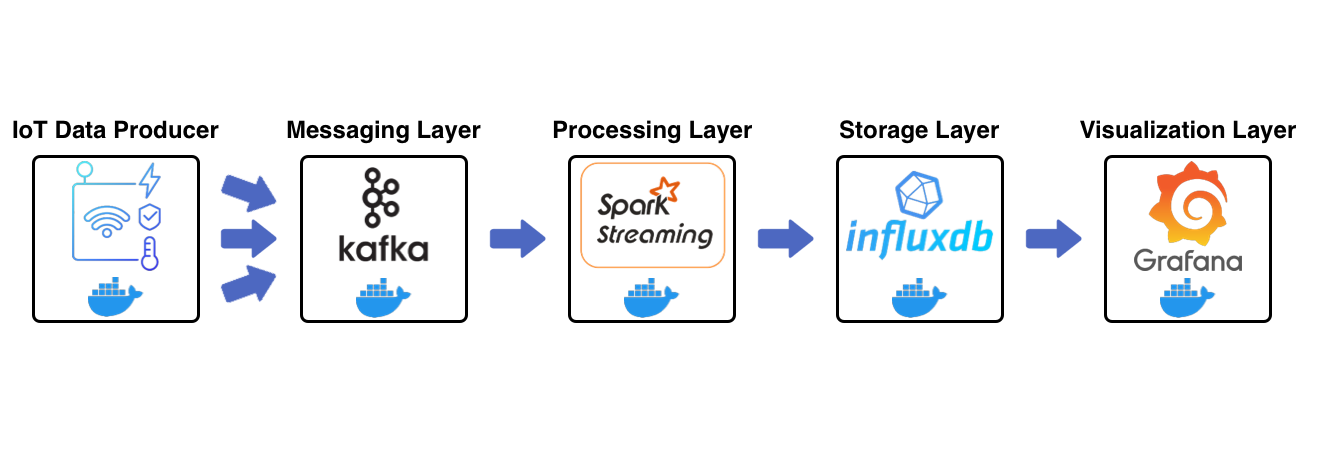
\includegraphics[width=1\linewidth]{Schema-Architettura-1}
\centering
\caption*{Rappresentazione schematica architettura sistema}
\label{fig:bytepost}
\end{figure}

\bigskip
\noindent
Come rappresentato nella figura precedente, il sistema è composto principalmente da 5 blocchi:
\begin{itemize}[noitemsep]
  \item \textbf{IoT data producer}: sensori installati nel campo di peschi, i quali rilevano dati con una diversa frequenza, come riportato in precedenza nel capitolo 1, che vengono inviati al blocco successivo. Come detto in precedenza, non avendo acceso diretto ai sensori e avendo a disposizione file JSON con i dati raccolti, in questo blocco è stato simulato l'invio dei dati dai sensori.
  \item \textbf{Messaging Layer}: si occupa di memorizzare i dati provenienti dai sensori e li fornisce al blocco successivo.
  \item \textbf{Processing Layer}: processa in real time i dati provenienti dal messaging layer.
  \item \textbf{Storage Layer}: memorizza i dati processati dal blocco precedente.
  \item \textbf{Visualizzation Layer}: visualizza i dati salvati in real time.
\end{itemize}
Grazie a docker, i cinque blocchi sono stati fatti partire su 5 container separati. \\
Per il primo blocco, relativo alla simulazione dei sensori IoT, è stato creato un Dockerfile nel quale è stato definito il container e successivamente è stata creata l'immagine contenente il container. Per gli altri blocchi sono state utilizzate delle immagini di container già esistenti nel \href{https://hub.docker.com} {\textbf{Docker Hub Container Image Library}}.\\
Le variabili d'ambiente necessarie per il corretto funzionamento dei container sono state definite all'interno del file \texttt{docker-compose.yml}.\\
Una volta scaricate le immagini dei container e definite le variabili d'ambiente, il tutto è stato fatto partire con lo script \texttt{start-compose.sh} presente all'interno della cartella \textit{script}. Nella stessa cartella è presente anche lo script \texttt{stop-compose.sh} per interrompere l'esecuzione dei container.

\subsection{Dati da sensori IoT}
Il primo container realizzato è stato quello per i sensori IoT. Come riportato in precedenza, non avendo accesso diretto ai sensori l'invio dei dati è stato simulato mediante un container docker. I file e gli script necessari per il funzionamento del seguente container sono presenti all'interno della cartella \textit{iot-data-producer}.\\
Il container è stato definito all'interno del file \textbf{Dockerfile}. Per leggere i dati e trasmetterli al messaging layer (realizzato usando Kafka), è stato utilizzato uno script Python, quindi nel Dockerfile è stata definita l'ultima versione di Python da installare nel container e il package \textit{kafka-python} che consiste in un client Kafka per il linguaggio Python, il quale permette allo script di interagire con Kafka.
Una volta definito il file Dockerfile, l'immagine del container è stata generata mediante lo script \textit{build-iot-container} presente all'interno della cartella script.\\
Lo script Python realizzato per leggere ed inviare i dati a Kafka, prende in input il nome del file in formato JSON da leggere e inizializza il producer per inviare i dati al container nel quale è in esecuzione Kafka (raggiungibile all'endpoint \textit{kafka:9093}). Successivamente legge il file JSON, inizializza le chiavi presenti nel file in una lista e scorre i valori delle chiavi al contrario (questo perchè l'ultima riga è il dato memorizzato più recente). Come visto in precedenza il file ha per ogni chiave un valore e un timestamp. La chiave rappresenta i diversi dati raccolti da un unico sensore, quindi nello stesso istante di tempo il sensore invia più dati. Lo script effettua anche dei controlli sul nome delle chiavi e sul nome del file perchè ci possono essere sensori chiamati uguali, che inviano dati con le stesse chiavi ma che possono essere installati su punti diversi. Quindi, per ogni riga di ogni chiave del file vengono generate due liste nelle quali, in una vengono inserite le chiavi e nell'altra, seguendo lo stesso ordine, vengono inseriti i valori. Il timestamp essendo lo stesso viene inserito in una variabile. Dalle due liste e dal valore del timestamp viene generato un messaggio convertito in una stringa JSON. \\
Il producer definito in precedenza si occupa di inviare il messaggio contenente la stringa JSON e il nome del file letto a Kafka. I dati vengono inviati a Kafka ad intervalli di 5 secondi. Il nome del file letto viene utilizzato da Kafka per creare topic differenti sui quali andare a memorizzare i messaggi provenenti dal seguente container. In questo caso sono stati definiti 10 topic avendo a disposizione 10 file differenti.\\
L'invio in parallelo dei dati da tutti i sensori è stato realizzato mediante lo script \textit{start-producer.sh} presente all'interno della cartella script, che richiama per ogni file JSON lo script Python descritto e al quale viene passato il nome di ogni file. 

\subsubsection{Pseudocodice}
% IoT data producer
\begin{algorithm}[H]
  \caption{IoT data producer}
  $\var{IOT\_NAME} \assign \text{None}$\;
  \Function{generate\_messages($keys$, $timestamp$, $values$)}{
  	$\var{messages} \assign \text{\{"key": keys, "value": values, "ts": timestamp\}}$\;
	 \Return{$\text{json.dumps(messages).encode('UTF-8')}$}\;
  }
  \Comment{The main function}
   \If{$\var{\_\_name\_\_}$ EQUALS  \textit{\_\_main\_\_}}{
   	$\var{IOT\_NAME} \assign \text{sys.argv[1]}$\;
  	$\var{producer} \assign \FuncCall{KafkaProducer}{$bootstrap\_servers=kafka:9093$}$\; 
	
	\With{$\var{open(jsonFile)}$} {
		$\var{data} \assign \text{load json file}$\;
		$\var{keys} \assign \text{data keys}$\;
		\For {$\var{i}$ in \text{reversed range of data}} {
			$\var{values} \assign \text{[ ]}$\;
			$\var{timestamp} \assign \text{timestamp row i}$\;
			$\var{new\_keys} \assign \text{[ ]}$\;
			\For {$\var{key}$ in $\var{keys}$} {
				$\text{values append data[key][i] value}$\;
			}
			$\var{producer.} \texttt{send(IOT\_NAME, }$\;
			\qquad \qquad \FuncCall{generate\_messages}{$new\_keys$, $timestamp$, $values$}\;
			$\var{time.} \FuncCall{sleep}{$5$}$
		}
	}
    }
\end{algorithm}

\subsubsection{Log - Output}
\begin{figure}[H]
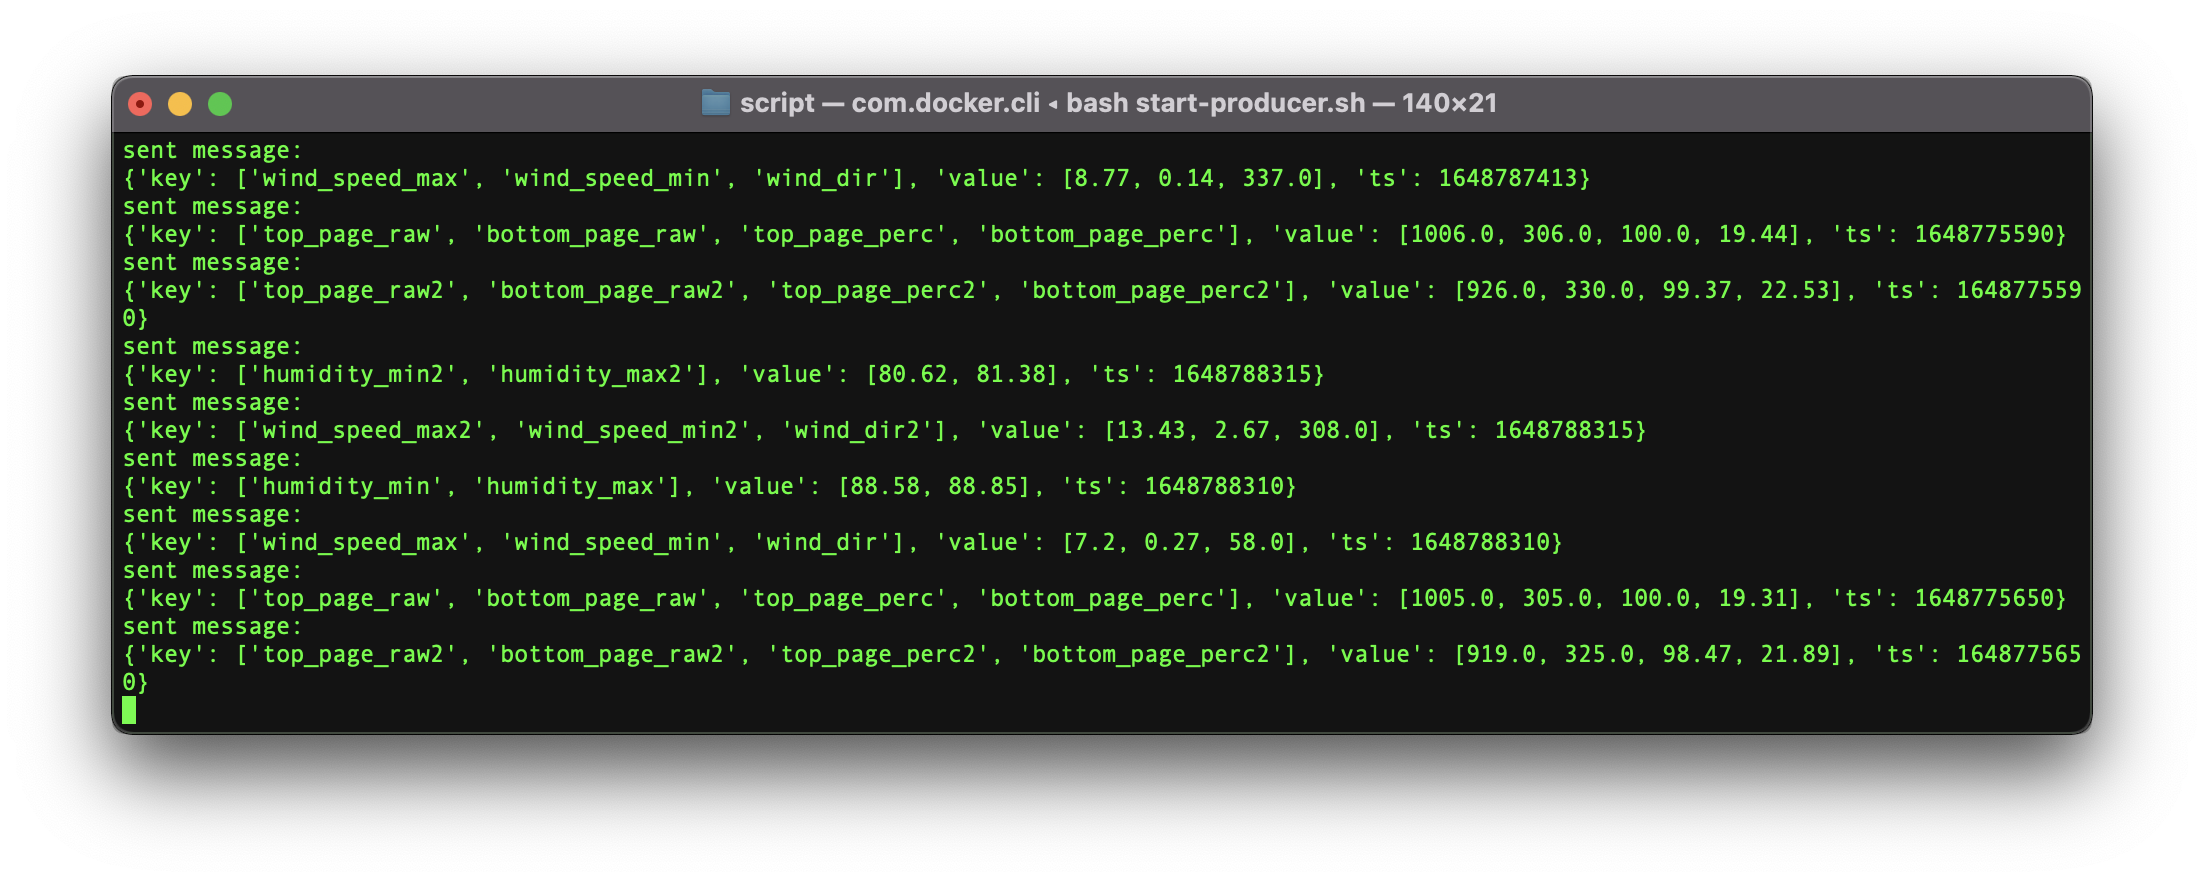
\includegraphics[width=1\linewidth]{Output-producer}
\centering
\caption*{Output script iot-producer}
\label{fig:bytepost}
\end{figure}

\subsection{Messaging Layer}
I messaggi generati e trasmessi attraverso lo script Python descritto in precedenza arrivano al messaging layer, realizzato con Kafka. Il vantaggio di usare un blocco intermedio tra i produttori di dati (sensori IoT) e i consumatori (Spark Streaming) sta nella possibilità di disaccopiare gli uni dagli altri. Ad esempio, grazie a questo strato intermedio, sarebbe possibile utilizzare una diversa tecnologia per processare gli stream di dati prodotti dai sensori (ad esempio Apache Storm) senza che questo abbia alcun impatto sui produttori di dati. In assenza di Kafka sarebbe stato necessario configurare i sensori affinché inviassero dati al cluster su cui è in esecuzione Spark Streaming oppure Apache Storm.\\
I messaggi prodotti dallo script Python vengono trasmessi e memorizzati in un container su cui è in esecuzione Kafka.
In particolare i messaggi provenienti da diversi sensori, in questo caso da diversi file, vengono memorizzati in \textit{topic} differenti. I topic prendono il nome del file letto e occorre definirli nello script del successivo layer per permettere a Spark di leggere i messaggi. Inoltre, è stata definita la variabile d'ambiente \texttt{KAFKA\_AUTO\_CREATE\_TOPICS\_ENABLE=true} che permette a Kafka di generare automaticamente i topics dal messaggio che viene inviato.\\ 
Occorre ricordare che per poter funzionare Kafka ha bisogno Zookeeper, il quale è un servizio di sincronizzazione per grandi sistemi distribuiti. Nel seguente progetto Zookeeper è stato configurato ed eseguito su un altro container raggiungibile all'endpoint \textit{zookeeper:2181} e per il corretto funzionamento di Kafka è stata aggiunta la variabile d'ambiente \texttt{KAFKA\_ZOOKEEPER\_CONNECT=zookeeper:2181} che permette a Kafka di collegarsi al container nel quale è in esecuzione Zookeeper.

\subsection{Processing Layer}
I dati memorizzati su Kafka vengono inviati ad un cluster di container Spark composto da un container master e da un container worker. Per processare i dati è stato utilizzato Spark Streaming. Lo script è stato scritto in Python. Nello script è stata inizializzata la SparkSession e sono stati definiti i topic da leggere. Lo script si mette in ascolto del container Kafka (kafka:9093) e quando il container dei sensori invia un nuovo dato, Kafka trasmette il messaggio e viene letto lo streaming di dati. I dati vengono salvati su un DataFrame e per poter ottenere le chiavi, i valori e il timestamp occorre effettuare una decodifica del DataFrame. Per questa operazione è stato definito un \textit{messageSchema} che descrive con i tipi i campi del messaggio ricevuto e ne permette la decodifica.\\
I dati ricevuti vengono letti in batch di diversa dimensione e in un batch possono essere presenti dati provenienti da più sensori. Per questo motivo viene eseguito un foreach per ogni batch ricevuto e viene richiamata la classe \texttt{InfluxDBWriter}. I dati una volta processati vengono salvati su uno storage layer che consiste in un container su cui è installato InfluxDB. Il salvataggio dei dati prodotti avviene utilizzando il package Python \textit{influxdb\_client}.\\ 
La classe \texttt{InfluxDBWriter} si occupa di inizializzare la connessione con il database raggiungibile all'endpoint influx:8086 e di processare le righe del batch passate in input. Viene eseguito un controllo sulle chiavi che riceve e in base ad esse viene calcolato il valore medio. Ad esempio, nel caso delle chiavi: \texttt{wind\_speed\_min}, \texttt{wind\_speed\_max} e \texttt{wind\_dir}, viene calcolato il valore medio tra i valori \texttt{wind\_speed\_min} e \texttt{wind\_speed\_max}.\\
Inoltre, è stato inserito un controllo sul valore medio dell'umidità. Questo valore, insieme ai valori relativi alla bagnatura fogliare, devono essere tenuti sotto controllo perchè se superiori ad una certa soglia potrebbero provocare l'attacco di bolla sulle piante di pesco. Per le piante di pesco l'attacco di bolla è una delle malattie più diffuse. Nel seguente caso è stato inserito un valore di test per l'umidità perchè al momento non ci sono abbastanza dati per stabilire con certezza le soglie dei valori.
Come si può osservare in seguito dalla figura di output, se il valore dell'umidità è superiore la soglia viene stampato un messaggio di avviso in console. \\
Infine, i dati processati vengono salvati sullo storage layer.\\
Per poter installare il package \textit{influxdb\_client} nel container Spark e lanciare il seguente script Python è stato utilizzato lo script \textit{start-spark.sh} presente all'interno della cartella script.

\subsubsection{Pseudocodice}
% Spark-app
\begin{algorithm}[H]
  \caption{Spark-app}
  \Class{InfluxDBWriter}{
  	\Function{\_\_init\_\_($\texttt{self}$)}{
  		$\var{self.\_token} \assign \var{token}$\;
		$\var{self.\_org} \assign \textit{'primary'}$\;
		$\var{self.client} \assign \FuncCall{InfluxDBClient}{$'influx:8086'$, $self.\_token$, $self.\_org$}$\;
		$\var{self.write\_api} \assign \var{self.client.write\_api()}$\;
	 }
	 \Function{open($\texttt{self, partition\_id, epoch\_id}$)}{
		\texttt{Output(}\textit{'Opened:'} \texttt{partition\_id, epoch\_id)}\;
		\Return{True}
	 }
	 \Function{process($\texttt{self, row}$)}{
  		$\var{self.write\_api.write(} \textit{'primary'} \var{, self.\_row\_to\_line\_protocol(row))}$\;
	 }
	 \Function{close($\texttt{self, error}$)}{
  		$\var{self.write\_api.\_\_del\_\_()}$\;
  		$\var{self.client.\_\_del\_\_()}$\;
		\texttt{Output(}\textit{'Close with error:'} \texttt{error)}
	 }
	 \Function{\_row\_to\_line\_protocol($\texttt{self, row}$)}{
	 	\Comment{Check key and value for all generated data from iot script}
	 	\If{$\var{row['key']}$ EQUALS  \text{key from iot script}}{
			\If{$\var{row['value']} \ge \text{value}$}{
				\texttt{Output(Warning value!)}
			}
		\Return{$\text{save data on database}$}\;
		}
	 }
  }
  \Comment{The main function}
   \If{$\var{\_\_name\_\_}$ EQUALS  \textit{\_\_main\_\_}}{
   	$\var{spark} \assign \text{initialize the SparkSession}$\;
  	$\var{df} \assign \text{read Kafka stream}$\;
	$\var{df1} \assign \text{get values from df json}$\;
	$\var{df1.writeStream.foreach(InfluxDBWriter())}$\; 
    }
\end{algorithm}

\subsubsection{Log - Output}
\begin{figure}[H]
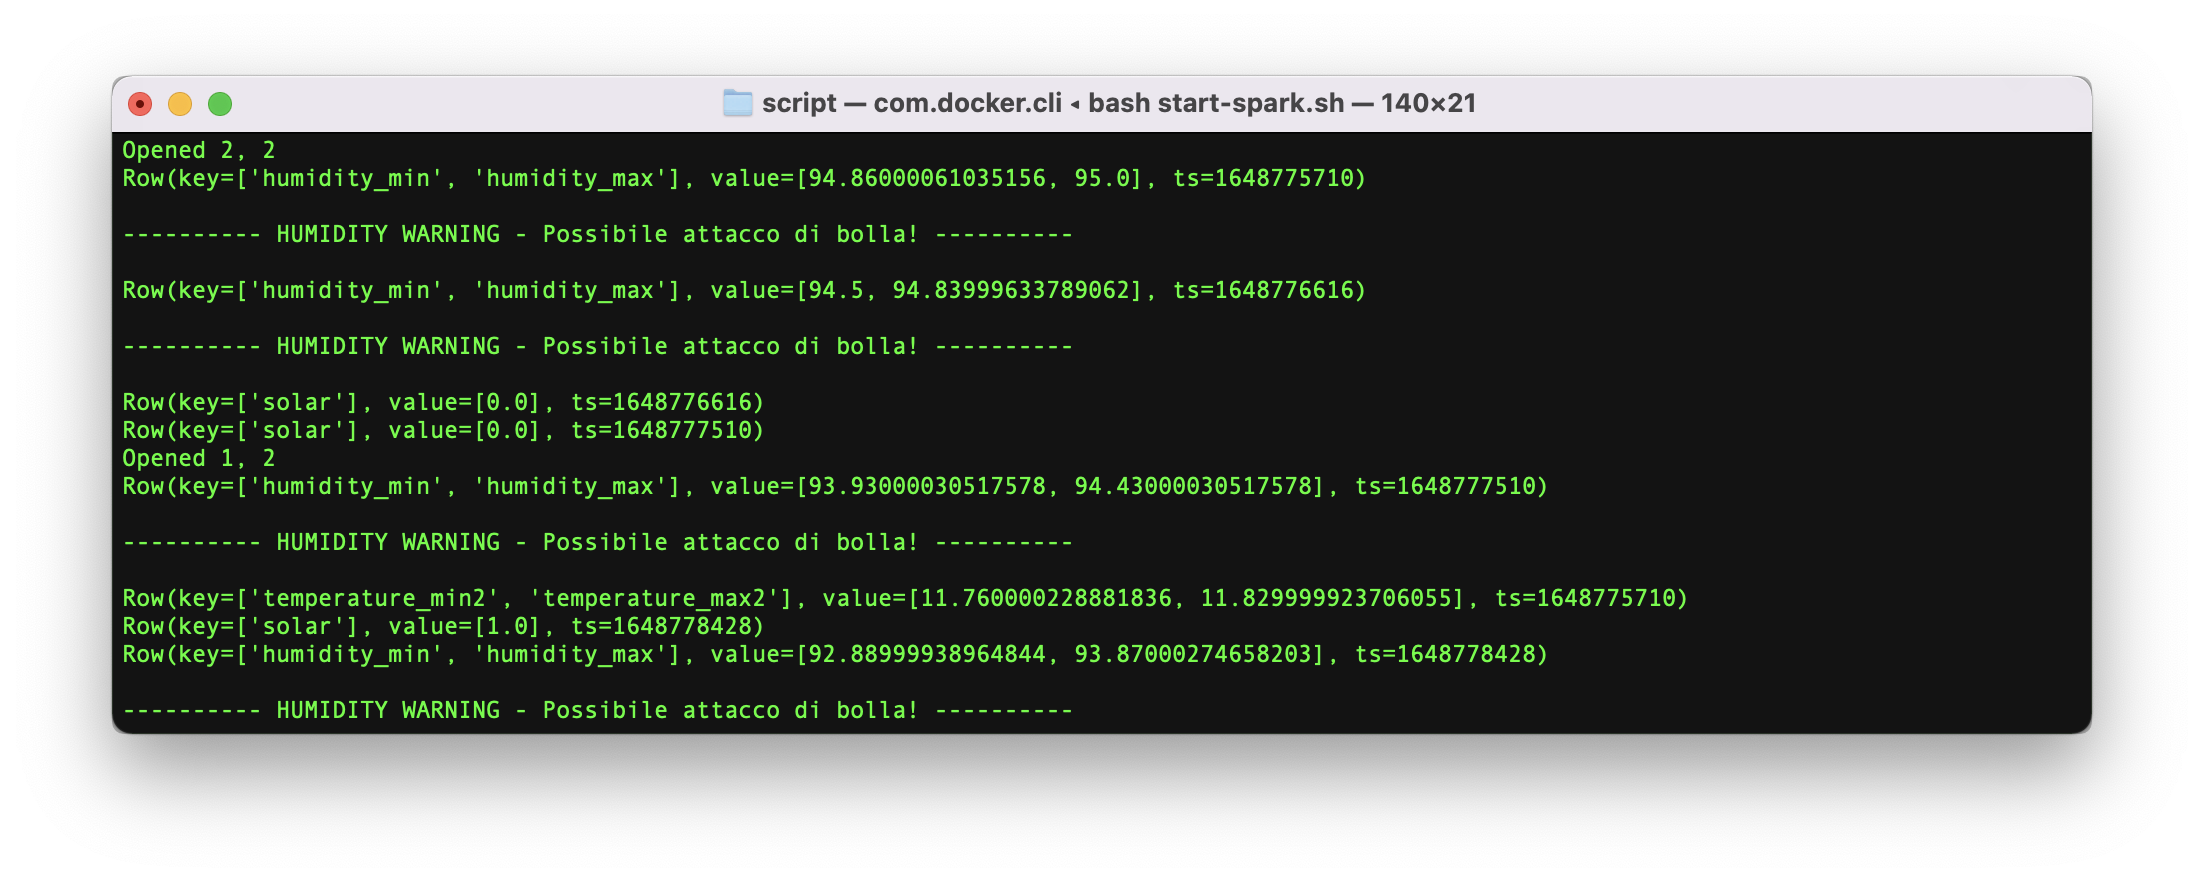
\includegraphics[width=1\linewidth]{Output-spark-1}
\centering
\caption*{Output spark script}
\label{fig:bytepost}
\end{figure}

\begin{figure}[H]
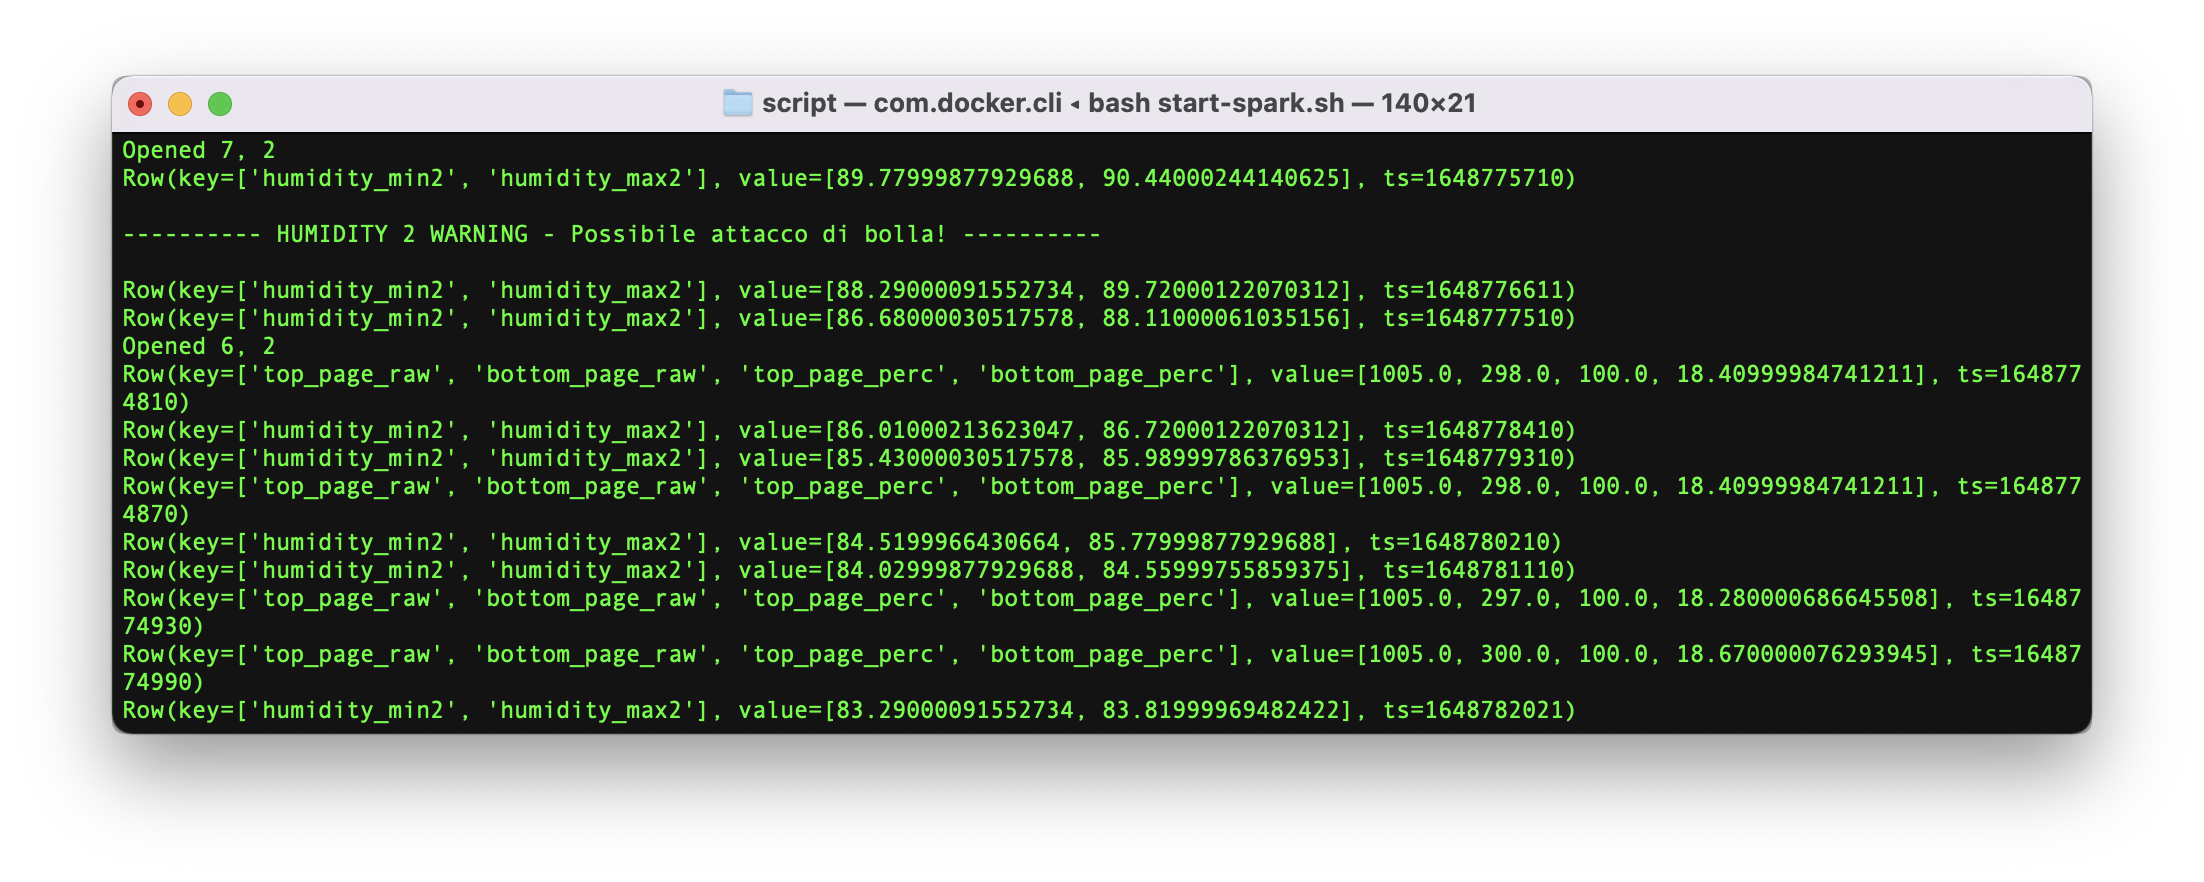
\includegraphics[width=1\linewidth]{Output-spark-2}
\centering
\caption*{Output spark script}
\label{fig:bytepost}
\end{figure}


 
\subsection{Storage Layer}
I dati processati da Spark Streaming vengono salvati all'interno di InfluxDB. 
InfluxDB è un base di dati che appartiene alla categoria dei \textit{Time Series Database (TSDB)}, ovvero una tipologia di database ottimizzati per \textit{time series data}. I time series data sono dati o eventi che vengono registrati, aggregati e monitorati nel tempo, come ad esempio la quantità di CPU e RAM usata in un server, i dati provenienti da sensori e così via.
In un Time Series Database i dati memorizzati sono associati ad un timestamp e questa tipologia di database è ottimizzato per misurare i cambiamenti nel tempo di una data metrica (come ad esempio la percentuale di CPU utilizzata nell'esempio precedente).\\
Nel seguente progetto i dati di partenza provengono da sensori e sono associati tutti ad un timestamp e per questo si è scelto di utilizzare un Time Series Database (TSDB) per memorizzare i dati prodotti da Spark Streaming.
Nel panorama dei TSDB la scelta è poi ricaduta su InfluxDB perchè è compatibile con Grafana per la visualizzazione dei dati (descritto nella sezione successiva) e perchè tra i Time Series Database, secondo DB-Engines, si classifica al primo posto.

\begin{figure}[H]
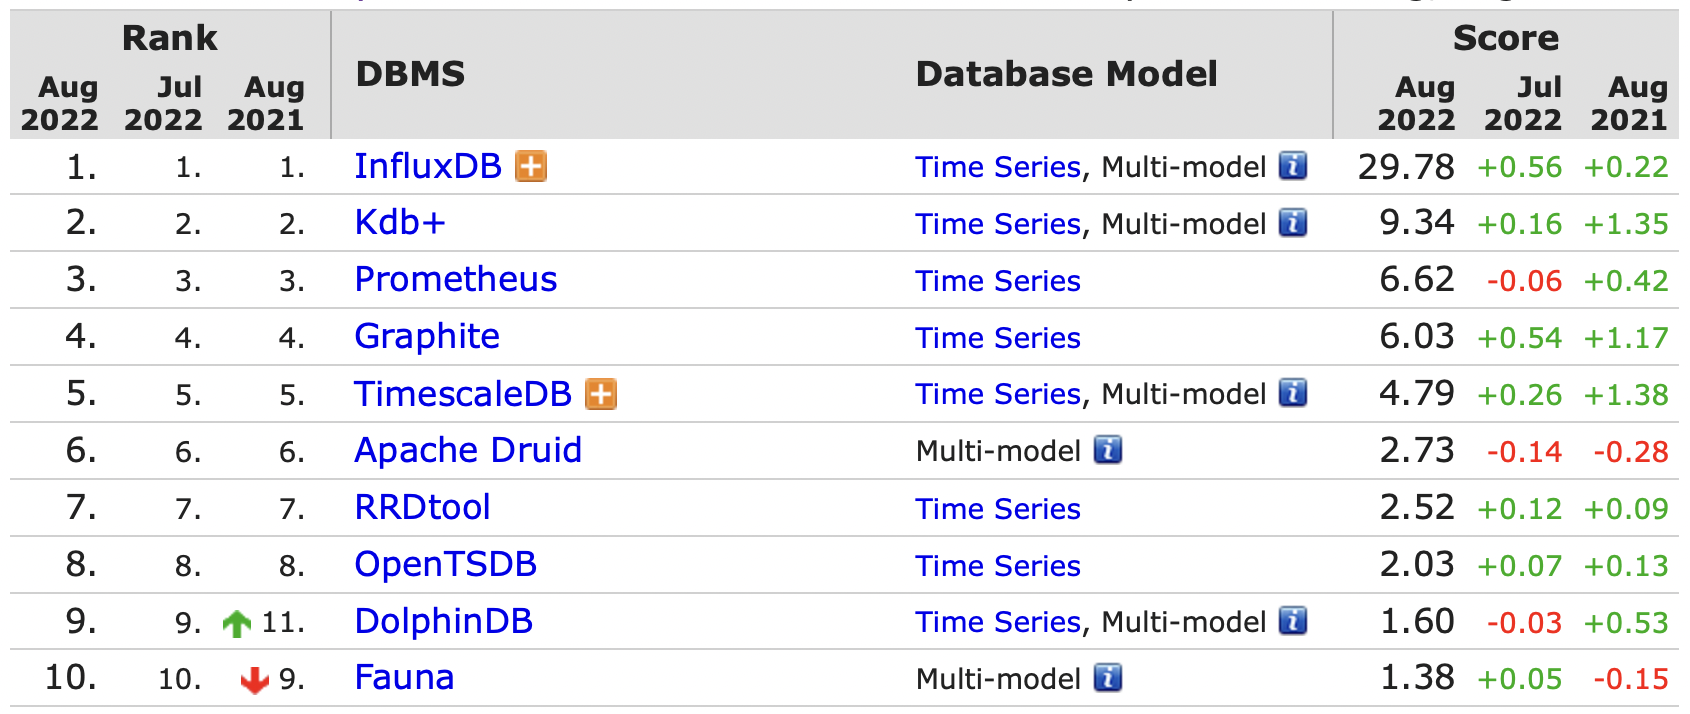
\includegraphics[width=1\linewidth]{Database-Rank}
\centering
\caption*{Ranking dei TSDMB secondo DB-Engines}
\label{fig:bytepost}
\end{figure}

\bigskip
\noindent
Concetti di base di InfluxDB:
\begin{itemize}[noitemsep]
    \item \textit{Measurement}, che corrisponde al concetto di \textit{tabella} in un RDBMS;
    \item \textit{Tag}, che può essere visto come una colonna indicizzata in un RDBMS;
    \item \textit{Field}, che corrisponde al concetto di colonna (non indicizzata) in un RDBMS;
    \item \textit{Point}, che corrisponde al concetto di riga in un RDBMS.
\end{itemize}

\smallskip
\noindent
Si riporta di seguito una sequenza di dati di esempio rappresentati sia in un RDBMS che in InfluxDB:
\begin{figure}[H]
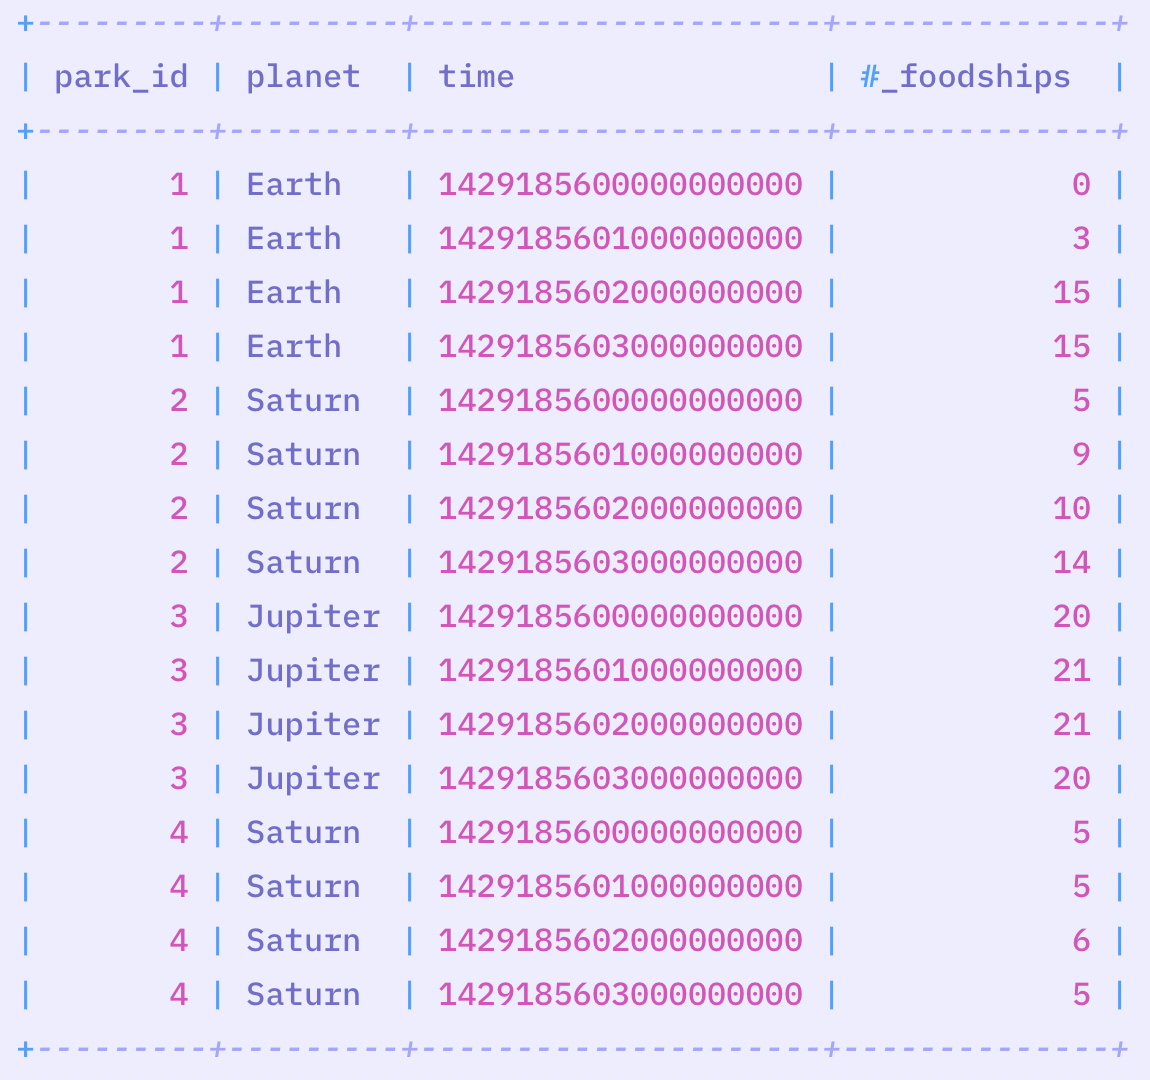
\includegraphics[width=0.55\linewidth]{Data-RDBMS}
\centering
\caption*{Dati rappresentati in un RDBMS}
\label{fig:bytepost}
\end{figure}

\begin{figure}[H]
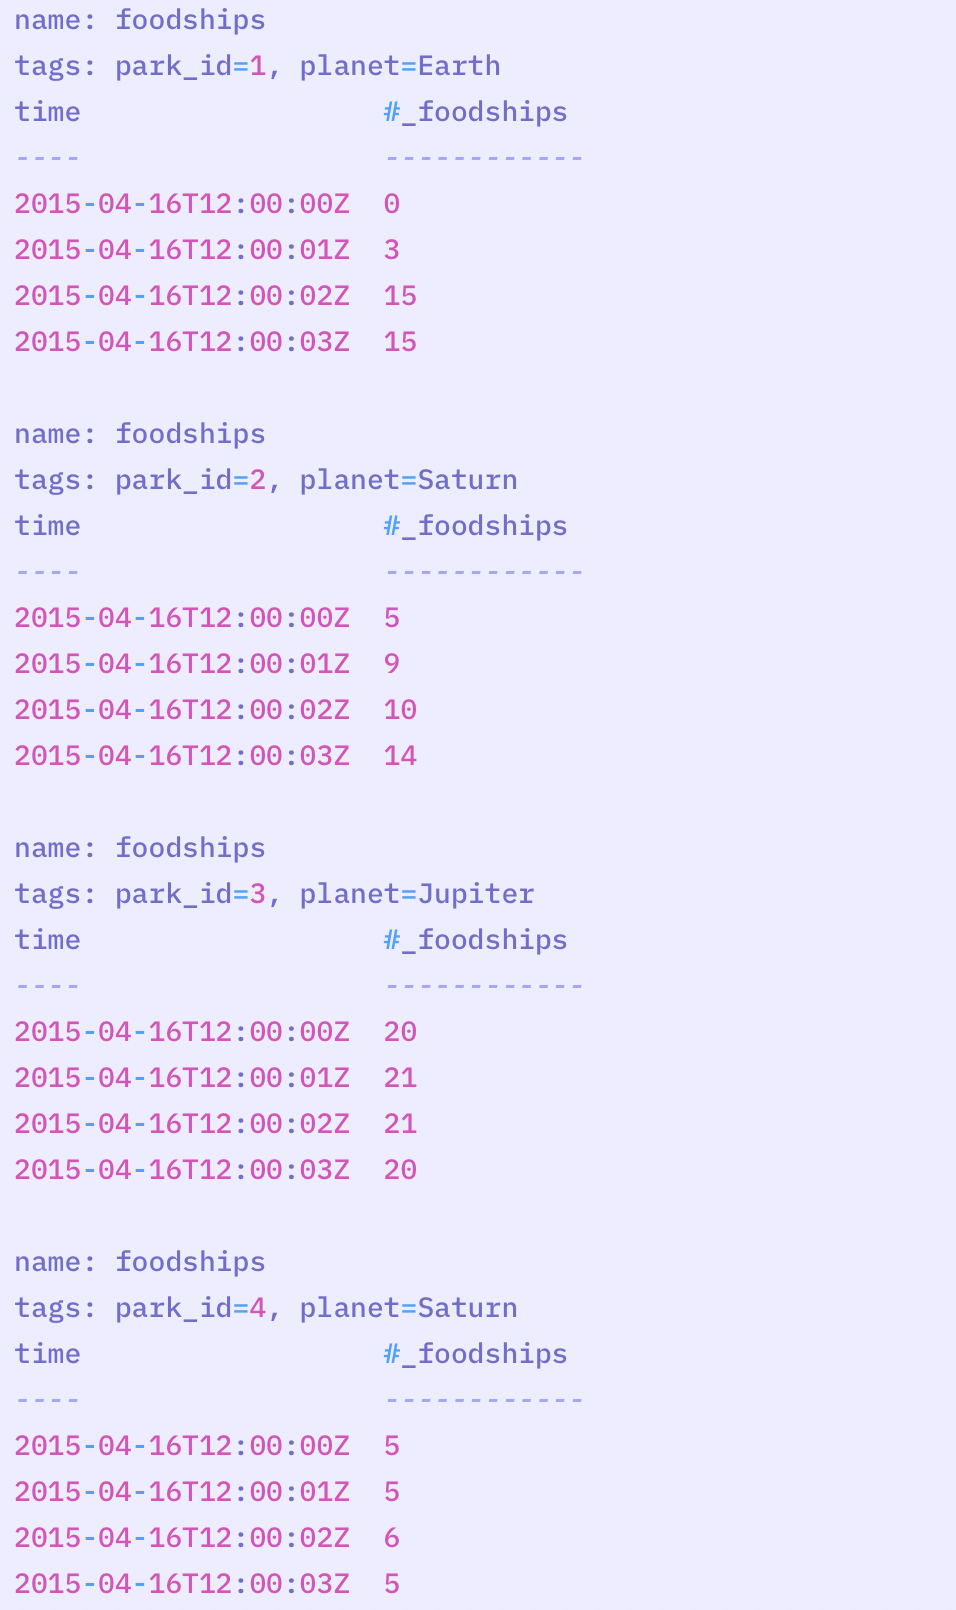
\includegraphics[width=0.55\linewidth]{Data-InfluxDB}
\centering
\caption*{Dati rappresentati in un InfluxDB}
\label{fig:bytepost}
\end{figure}

\smallskip
\noindent
Con riferimento ad InfluxDB in questo esempio:
\begin{itemize}[noitemsep]
    \item \texttt{foodship} corrisponde alla measurement;
    \item \texttt{park\_id} e \texttt{planet} sono i tag;
    \item \texttt{\#\_foodships} corrisponde ad un field.
\end{itemize}

\noindent
Per ciascuna riga è presente una colonna aggiuntiva, di nome \texttt{time} che rappresenta un timestamp associato alla riga in questione.\\

\noindent
I dati processati da Spark Streaming sono stati salvati per sensore ciascuno in una measurement distinto. A ciascun measurement è stato associato un tag identificativo e i field della measurement corrispondono ai dati processati con Spark Streaming. Nel caso della measurement \textit{wind\_speed}, i field sono: \textit{Max}, \textit{Mean}, \textit{Min} e \textit{Dir}. \\
Tutti i dati sono stati salvati all'interno del bucket \textit{primary}. Un bucket è la posizione dove vengono archiviati i dati delle serie temporali.
Inoltre, sono state definite alcune variabili d'ambiente all'interno di \textit{docker-compose.yml} necessarie per accedere al container di InfluxDB, per la scrittura dei dati e una volta salvati, alla lettura degli stessi.



\subsection{Visualization Layer}
L'ultimo layer si occupa della visualizzazione dei dati memorizzati su InfluxDB. In questo layer è stato utilizzato Grafana.\\ 
Grafana è uno strumento di visualizzazione di serie temporali, accessibile tramite browser, che supporta una serie di database da cui leggere i dati quali \textit{Graphite}, \textit{MySQL}, \textit{PostgreSQL}, \textit{ElasticSearch} e molti altri oltre al già citato InfluxDB.
In particolare, grazie a Grafana è stata realizzata una \textit{dashboard} in cui sono state riportate le serie temporali associate ai sensori con i dati processati tramite Spark Streaming e memorizzati in InfluxDB. Nella dashboard sono stati inseriti 10 grafici, uno per ogni sensore, nei quali è possibile visualizzare i dati.\\
Per poter accedere ai dati e visualizzarli sono stati generati due file di configurazione presenti all'interno della cartella \textit{grafana/provisioring}. Nel file \textbf{datasource.yml} sono stati configurati i parametri per accedere ai dati memorizzati nel container di InfluxDB e nel file \textbf{dashboard.json} sono stati configurati i 10 grafici con le relative query per ottenere i dati.\\
Un esempio di query presente all'interno del file e utilizzata per ottenere il primo grafico riportato di seguito è:
\begin{lstlisting}[language=json,firstnumber=1]
{
"query": "from(bucket: \"primary\") 
|> range(start: 2022-04-01T01:00:00.000Z)
|> filter(fn: (r) => r._measurement == \"wind_speed\")"
}
\end{lstlisting}
La query seleziona dal bucket \textit{primary} tutti i dati relativi a \textit{wind\_speed} dalle \date{01:00} UTC del \date{2022-04-01}.

Una volta fatto partire il container è possibile visualizzare i grafici su qualsiasi browser raggiungibili all'indirizzo \texttt{localhost:3000}.

\newpage

\noindent
Si riporta di seguito istantanee della dashboard realizzata con i grafici:
\begin{figure}[H]
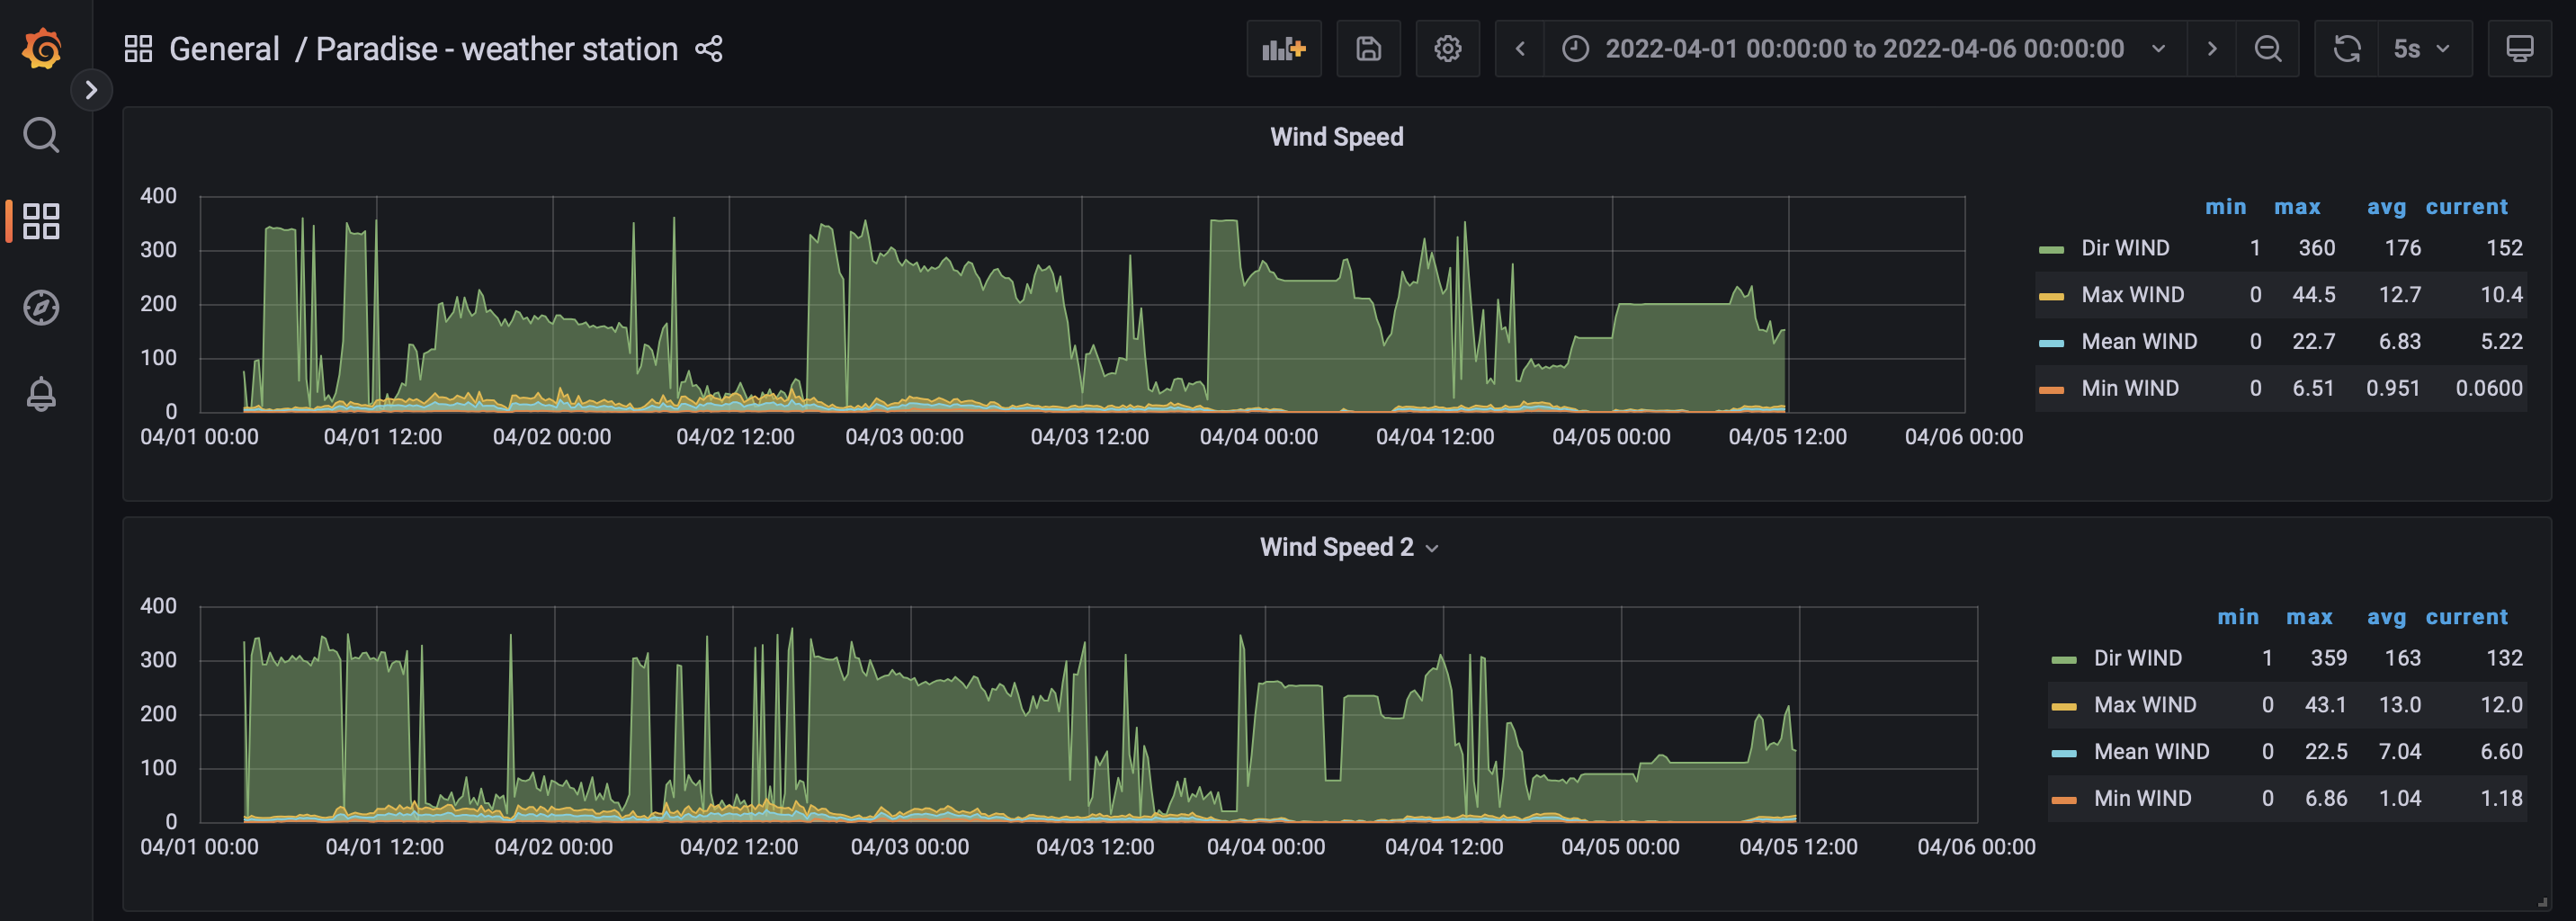
\includegraphics[width=1\linewidth]{WindSpeed-Graph}
\centering
\caption*{Sensori anemometri}
\label{fig:bytepost}
\end{figure}

\begin{figure}[H]
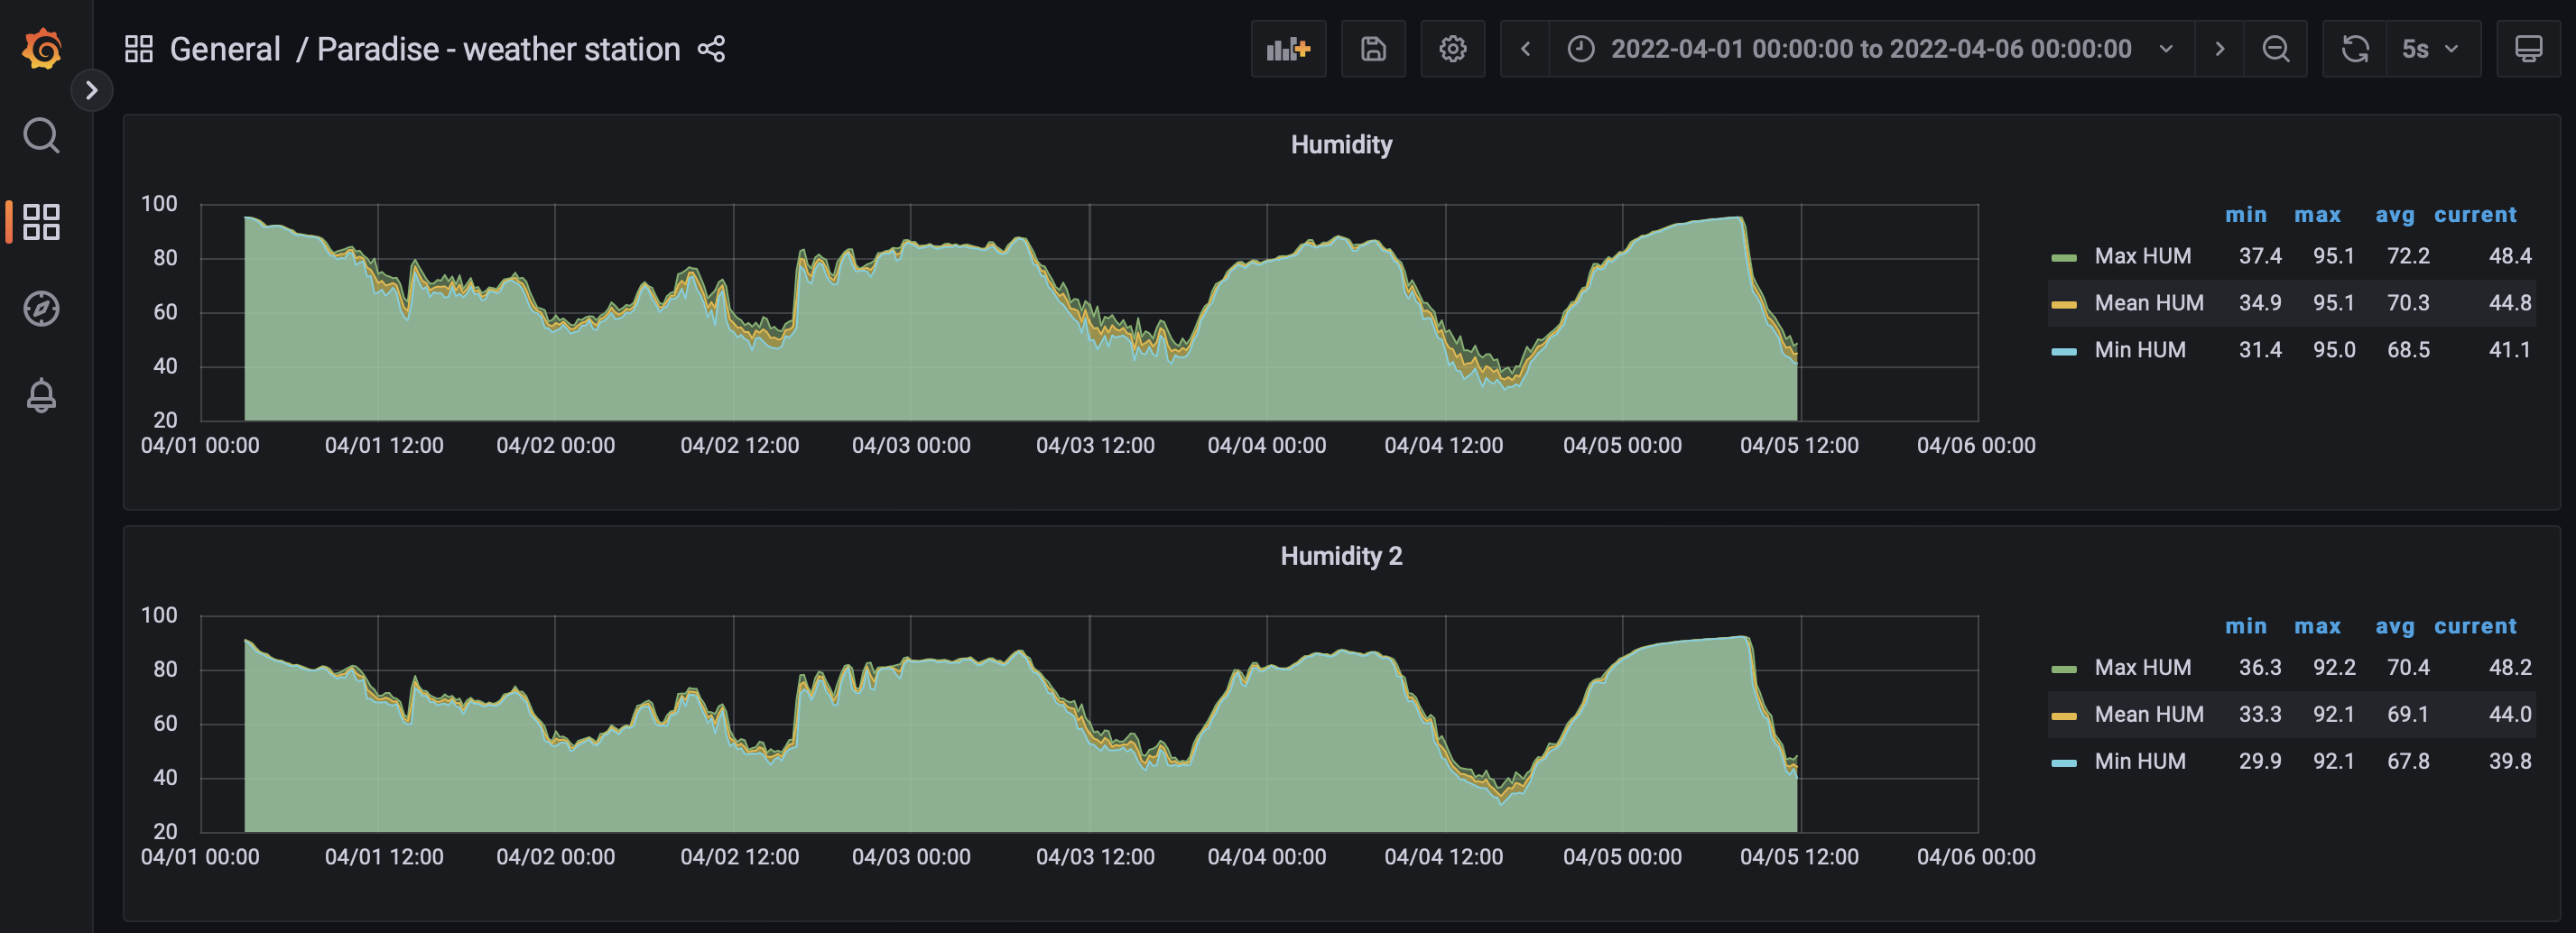
\includegraphics[width=1\linewidth]{Humidity-Graph}
\centering
\caption*{Sensori umidità}
\label{fig:bytepost}
\end{figure}

\begin{figure}[H]
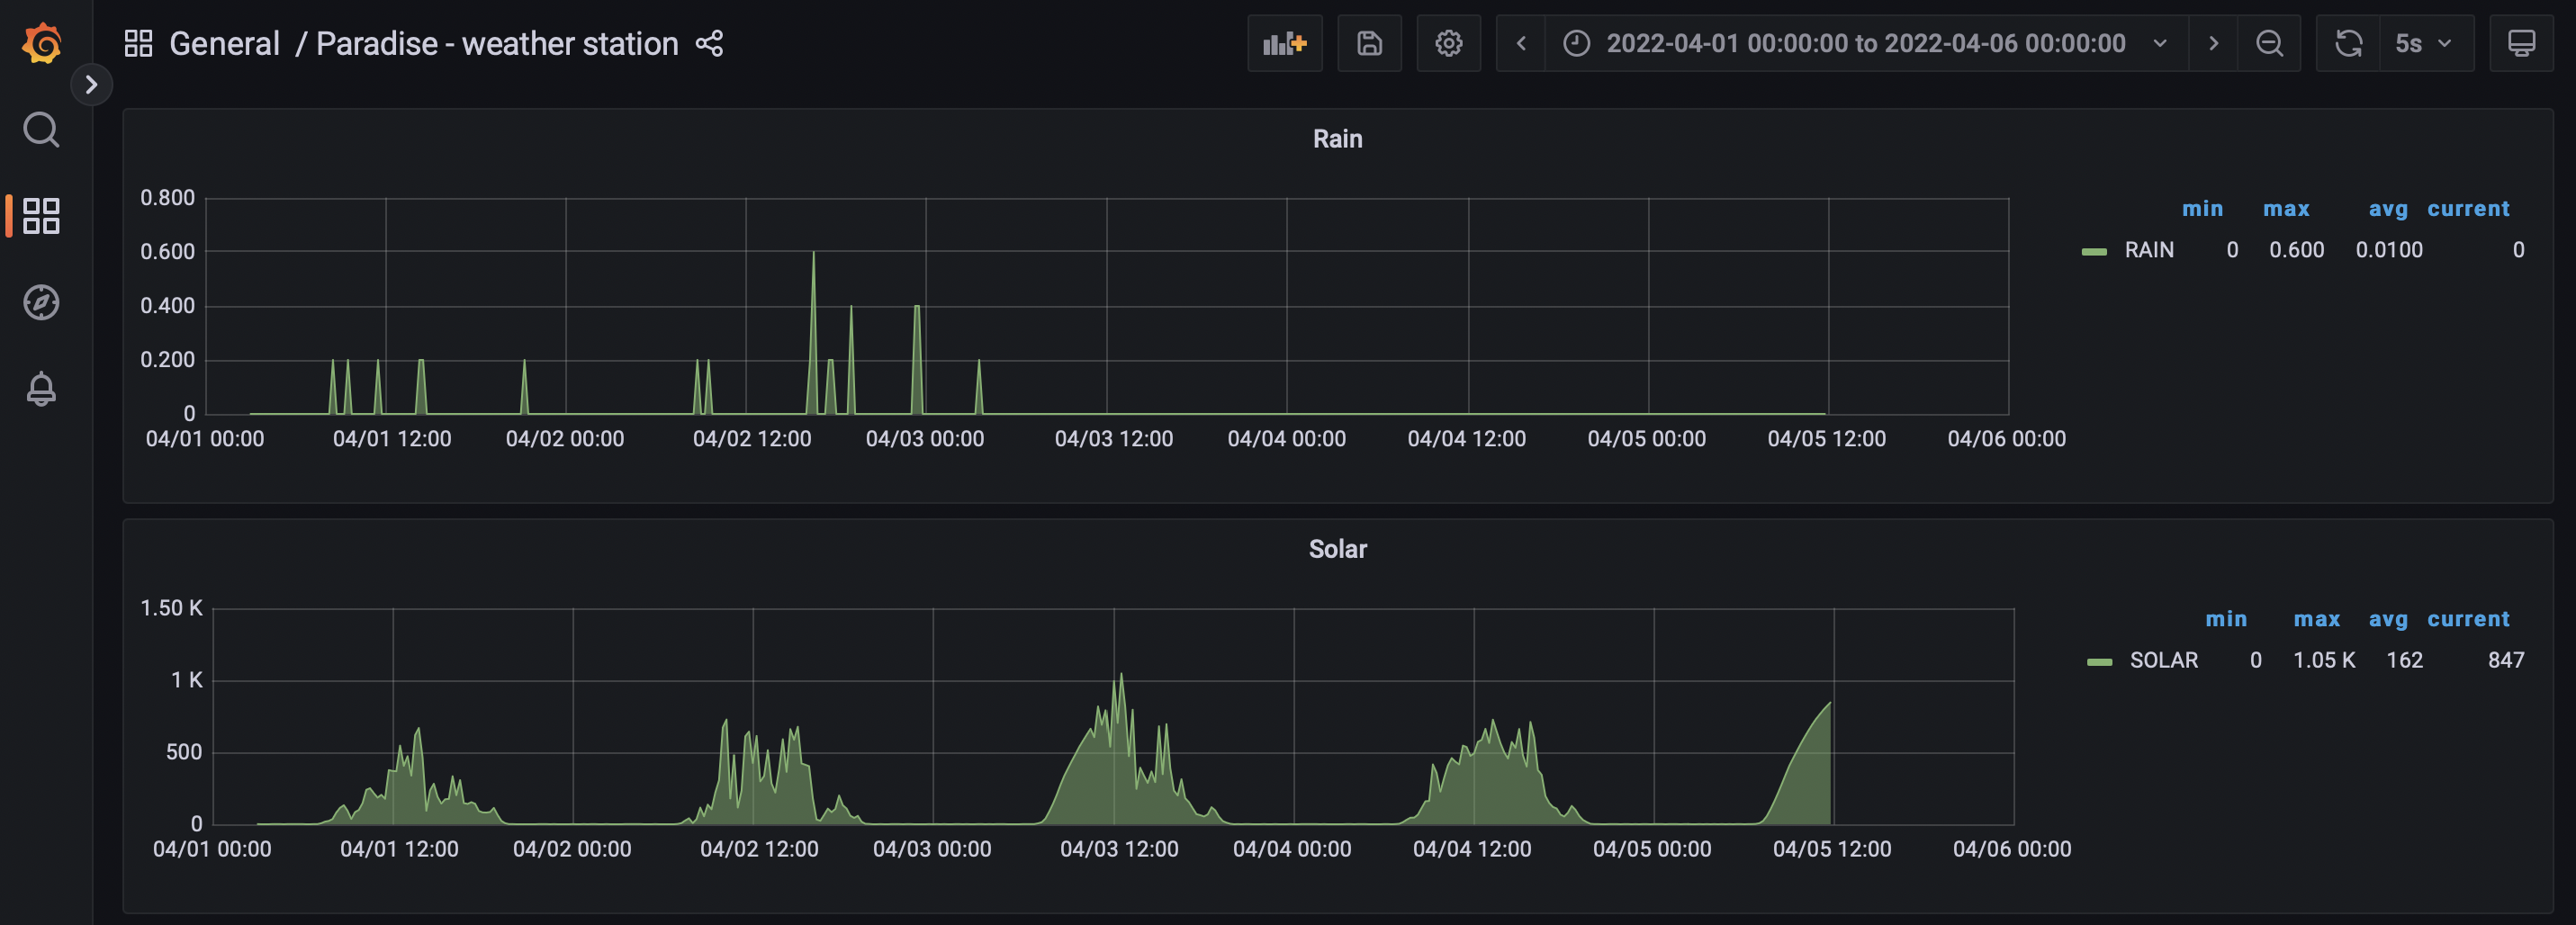
\includegraphics[width=1\linewidth]{Rain-Solar-Graph}
\centering
\caption*{Sensori pluviometro e radiometro}
\label{fig:bytepost}
\end{figure}

\begin{figure}[H]
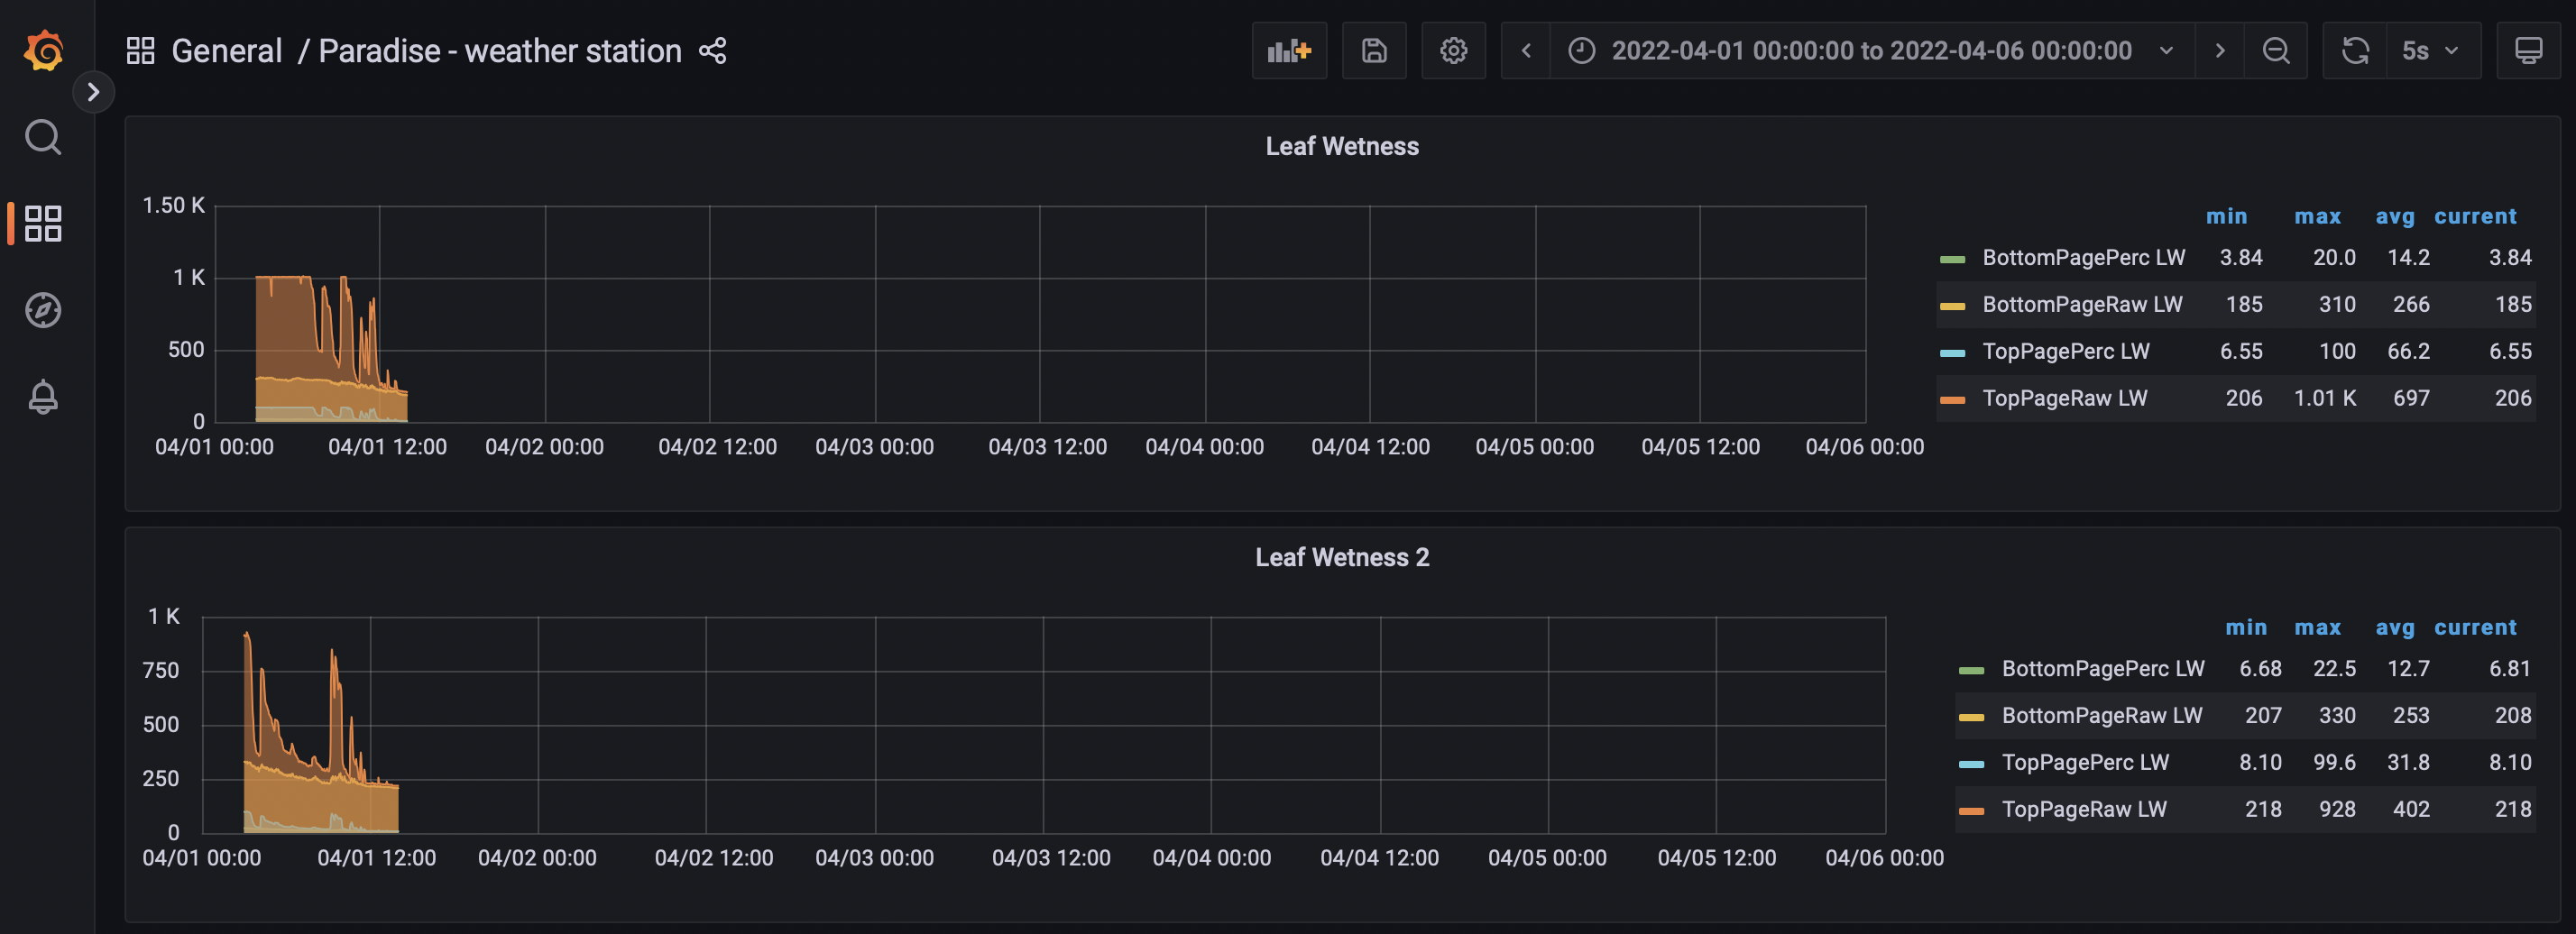
\includegraphics[width=1\linewidth]{LeafWetness-Graph}
\centering
\caption*{Sensori bagnatura fogliare}
\label{fig:bytepost}
\end{figure}

\begin{figure}[H]
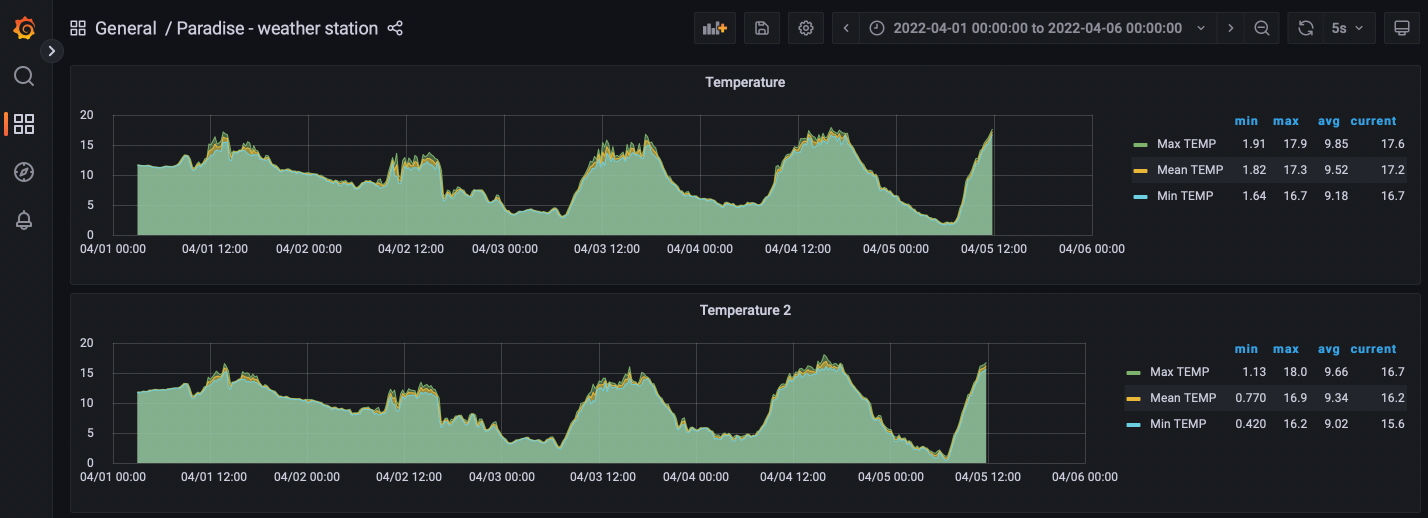
\includegraphics[width=1\linewidth]{Temperature-Graph}
\centering
\caption*{Sensori termo-igrometri}
\label{fig:bytepost}
\end{figure}

\noindent
Dai grafici si può osservare l'andamento dei dati raccolti, processati e memorizzati. In particolare, in ogni grafico è presente una sezione sulla parte destra del grafico che descrive i diversi dati raccolti in base al colore, ad esempio nell'ultimo grafico il colore verde rappresenta i dati relativi alla temperatura massima, ed è possibile selezionare un singolo dato e visualizzarne l'andamento. Sempre nella sezione a destra, per ogni dato visualizzato, è presente il valore minimo, massimo, medio e l'ultimo valore salvato.
Dalle istantanee sulla dashboard è possibile anche osservare che i grafici relativi al bagnatura fogliare sono in ritardo rispetto agli altri grafici, questo perchè, come detto in precedenza, i dati relativi alla bagnatura fogliare sono molti di più perchè vengono inviati ogni minuto, al contrario degli altri sensori che inviano dati ogni 15 minuti. \\
Inoltre, come riportato in figura sotto se viene passato il cursore del mouse sul grafico è possibile osservare nel dettaglio i valori nell'istante di tempo d'interesse.

\medskip
\begin{figure}[H]
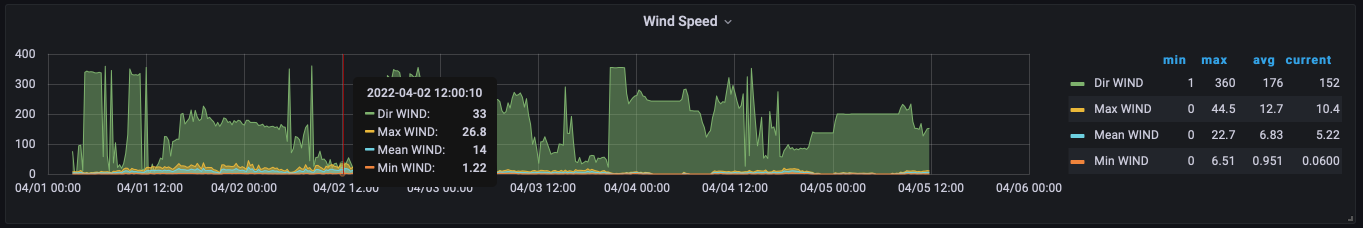
\includegraphics[width=1\linewidth]{Focus-Graph}
\centering
\caption*{Dettaglio valori grafico}
\label{fig:bytepost}
\end{figure}

\newpage

\section{Conclusioni e Sviluppi futuri}
In conclusione è stata realizzata un'architettura di big data per il monitoraggio in tempo reale di dati provenienti da sensori installati in un campo di peschi. Nel seguente caso non avendo a disposizione molti dati, l'attacco di bolla è stato simulato inserendo un valore di test, ma in futuro con molti più dati si potranno effettuare controlli molto più precisi. Oltre all'attacco di bolla si potranno verificare anche altri fattori che possono influenzare lo stato di salute delle piante.\\
Inoltre, si potrebbe inserire un nuovo layer nell'architettura per eseguire analisi batch dei dati e una possibile tecnologia da utilizzare potrebbe essere Apache Beam che offre un modello di processamento dei dati sia streaming che batch. \\
Con l'introduzione del layer per l'analisi batch, dai dati raccolti nell'analisi si potrebbe anche addestrare un modello di Machine Learning per contrastare problemi e malattie che possono influenzare lo stato di salute delle piante.

\newpage

\section{Riferimenti}
\begin{itemize}
    \item Documentazione Docker: \href{https://docs.docker.com}{\texttt{https://docs.docker.com}};
    \item Documentazione Docker Compose: \href{https://docs.docker.com/compose/}{\texttt{https://docs.docker.com/compose/}};
    \item Documentazione Kafka: 
    \begin{itemize}
    	\item Lezioni ed esercitazioni del corso di Big Data;
    	\item \href{https://kafka.apache.org/documentation/}{\texttt{https://kafka.apache.org/documentation/}};	
    \end{itemize}    
    \item Documentazione Spark Streaming: 
    \begin{itemize}
    	\item Lezioni ed esercitazioni del corso di Big Data;
    	\item \href{https://spark.apache.org/docs/latest/structured-streaming-programming-guide.html}{\texttt{Spark Structured Streaming Programming Guide}};	
    \end{itemize}    
    \item Documentazione InfluxDB: \href{https://docs.influxdata.com}{\texttt{https://docs.influxdata.com}};
    \item Documentazione Grafana: \href{https://grafana.com/docs/}{\texttt{https://grafana.com/docs/}}.
\end{itemize}





\end{document}